\documentclass[11pt,a4paper, final, twoside]{article}
%%%%%%%%%%%%%%%%%%%%%%%%%%%%%%%%%%%%%%%%%%%%%%%%%%%%%%%%%%%%%%%%%%%%%%%%%%%%%%%%%%%%%%%%%%%%%%%%%%%%%%%%%%%%%%%%%%%%%%%%%%%%%%%%%%%%%%%%%%%%%%%%%%%%%%%%%%%%%%%%%%%%%%%%%%%%%%%%%%%%%%%%%%%%%%%%%%%%%%%%%%%%%%%%%%%%%%%%%%%%%%%%%%%%%%%%%%%%%%%%%%%%%%%%%%%%
\usepackage{amsmath}
\usepackage{fancyhdr}
\usepackage{amsthm}
\usepackage{amsfonts}
\usepackage{amssymb}
\usepackage{amscd}
\usepackage{latexsym}
\usepackage{graphicx}
%\usepackage{graphics}
\usepackage{natbib}
\usepackage[colorlinks=true, urlcolor=blue,  linkcolor=black, citecolor=black]{hyperref}
\usepackage{color}
\usepackage{natbib}
\usepackage{sectsty}
\setcounter{MaxMatrixCols}{10}


\sectionfont{\fontsize{12}{15}\selectfont}

\renewcommand{\thefootnote}{}
\setlength{\oddsidemargin}{1pt} \setlength{\evensidemargin}{1pt}
\setlength{\hoffset}{-1in} \addtolength{\hoffset}{25mm}
\setlength{\textwidth}{140mm} 
\setlength{\marginparsep}{0pt} \setlength{\marginparwidth}{0pt}
\setlength{\topmargin}{0pt}
\setlength{\voffset}{-2in} \addtolength{\voffset}{20mm}
\setlength{\textheight}{300mm}
\setlength{\headsep}{20mm}
\setlength{\footskip}{15mm}
\pagestyle{fancy}
\fancyhead{} \fancyfoot{} 



%       Theorem environments
\newtheorem{thm}{Theorem}[section]
\newtheorem{algorithm}[thm]{Algorithm}
\newtheorem{axiom}[thm]{Axiom}
\newtheorem{lem}[thm]{Lemma}
\newtheorem{example}[thm]{Example}
\newtheorem{exercise}[thm]{Exercise}
\newtheorem{notation}[thm]{Notation}
\newtheorem{problem}[thm]{Problem}
\theoremstyle{proposition}
\newtheorem{prop}{Proposition}[section]
\newtheorem{case}[thm]{Case}
\newtheorem{claim}[thm]{Claim}
\newtheorem{conclusion}[thm]{Conclusion}
\newtheorem{condition}[thm]{Condition}
\newtheorem{conjecture}[thm]{Conjecture}
\newtheorem{cor}[thm]{Corollary}
\newtheorem{criterion}[thm]{Criterion}
\theoremstyle{definition}
\newtheorem{defn}{Definition}[section]
\theoremstyle{remark}
\newtheorem{rem}{Remark}[section]
\newtheorem{solution}[thm]{Solution}
\newtheorem{summary}[thm]{Summary}
\numberwithin{equation}{section}
\pagenumbering{arabic} % 1, 2, 3, 4, ...

\begin{document}
\hyphenpenalty=100000

\begin{center}
{\Large \textbf{\\A Feed-Forward Algorithm for Arithmetic Circuits}}\\[5mm]
{\large \textbf{Andrew Jemin Choi}\\[1mm]}
{\normalsize \emph{Under the supervision of Professor Guy Van den Broeck}\\[1mm]}
\end{center}

% Introduction
\section{Introduction}\label{I1}
Probabilistic queries are a foundation to many machine learning problems. We often query probabilistic models, such as Bayesian networks, to gain information about the variables in a system and make inferences about them. However, even the simplest queries in these networks, such as finding marginal probabilities of the input, come at an exponential cost. In fact, the problem of exact inference and making such queries in these probabilistic models is NP-hard. [1, 2]

An effective approach for making exact inferences in networks is to construct an Arithmetic Circuit (AC) from the network. [3] The state-of-the-art method uses a software algorithm to backpropagate the marginal probabilities of the AC. [4] We propose a new algorithm for calculating marginal probabilities by using feed-forward ACs, which can potentially reduce inference time and power comsumption. 

% Background
\section{Background}\label{I2}
A network polynomial is a linear function that outputs the probability of an event given the input parameters of the network. An example of one such polynomial is: \newline \centerline{$f=0.4\times(\theta_{f}) + 0.6\times(\theta_{\overline{f}})$} \newline
Evaluating the network polynomial is important in making inferences in our network. However, the number of terms in the polynomial is exponential with respect to the number of inputs. One compact way of representing these exponential terms is to express the polynomial using an arithmetic circuit. [2] 

An arithmetic circuit is a directed acyclic graph (DAG) whose leaves are variables or constants and whose interior nodes are addition or multiplication operations. The size of an arithmetic circuit is defined as the number of edges within the circuit. The size of the circuit also grows linearly with respect to the number of terms in the polynomial. 

% Diagram here
\begin{figure}[h]
    \caption{A binary arithmetic circuit that expresses the linear polynomial: $f=0.4\times(\theta_{f}) + 0.6\times(\theta_{\overline{f}})$}
    \centering
    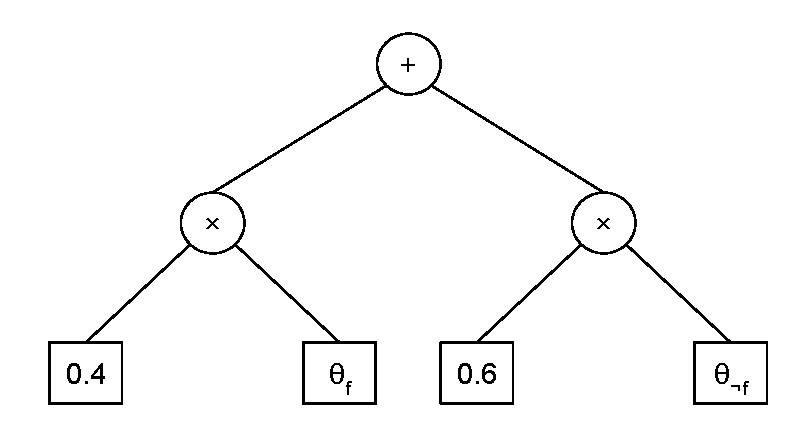
\includegraphics[width=9cm]{ac_example.pdf}
\end{figure}
\newpage
% End Diagram

By traversing the AC from the leaves, we can calculate the output of the polynomial at the root. Furthermore, if we start from the root, we can calculate the marginal probabilities by evaluating the partial derivatives for interior nodes, similar to how backpropation is used to update weights in a neural network. Both of these processes are linear in time with respect to the circuit size [2]. Similarly, the state-of-the-art uses a software implementation of bit-encoding backpropagation, where the original AC is traversed twice in order to find the marginal probabilities. One limitation to using bit-encoding is that it only works for alternating circuits, where every level of interior nodes alternate between addition and multiplication nodes.

% Approach
\section{Approach}\label{I3}
We propose a feed-forward approach to finding marginal probabilities. This approach would produce two arithmetic circuits, where the first circuit outputs the result of the polynomial and the second circuit outputs the marginal probability of a variable. By creating an additional circuit, we can perform additional optimizations and construct it in hardware to perform more efficient inferences.

% Diagram here
\begin{figure}[h]
    \caption{A high-level model of the proposed feed-forward AC}
    \centering
    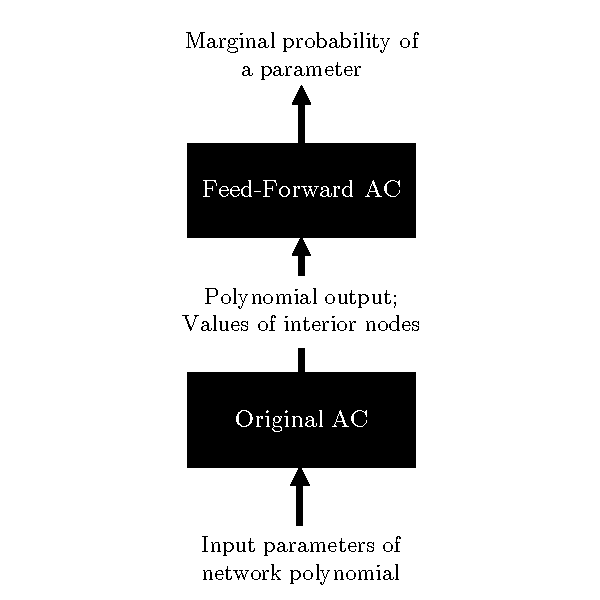
\includegraphics[width=10cm]{feedforward_example.pdf}
\end{figure}
\newpage
% End Diagram

Since partial derivatives of addition nodes are generally equal to the partial derivatives of the child nodes, we can calculate the partial derivatives by calculating the products of all sibling nodes of a child node, as follows: \newline\centerline{dr(c) = dr(p)$\times$ $\prod\limits_{c \neq c'}^{} vr(c')$ [4]}\newline where dr(c) is the derivative of the child node, dr(p) is the derivative of the parent node, and vr(c') is the value of a sibling node. This naive method requires many more edges than our original AC. As a result, the new AC will be quadratic in size with respect to our original AC using a naive approach.

Like the naive approach, our approach to finding marginal probabilities involves using only the product nodes; however, we do so i in a more efficient manner. We can do this by caching previously computed products and accessing them in future calculations, which is also a memoization technique. By caching the products into a register to calculate partial derivatives, the calculation can be done in linear size with respect to our original AC. 

This cache-based algorithm has two significant advantages compared to the bit-encoding algorithm:
\begin{enumerate}
\item The partial derivatives can be calculated in linear size, irrespective of the circuit structure. The feed-forward algorithm works correctly for non-alternating circuits, which is a feature absent from bit-encoded backpropagation. 
\item The algorithm can be used to create an external circuit that we can construct in hardware, which will allow us to perform additional optimizations to reduce inference time. 
\end{enumerate}

% Analysis
\section{Analysis}\label{I4}

We compared the performance of three algorithms, written in C, on three different data sets. For the feed-forward algorithm, we generated a feed-forward arithmetic circuit from the original circuit, and then compiled the circuit back into C code. Then, we measured the CPU time needed to find the marginal probability of one variable from the initialized circuit structures. 


 \begin{table}[h!]
 \centering
 \begin{tabular}{||c c c c ||} 
 \hline
 \textbf{Test Set} (nodes) & Bit-Encoded (s) & \textbf{Feed-Forward} (s) & Naive (s)\\ %[0.5ex] 
 \hline\hline
 \textbf{Verysimple.ac} (20) & 0.01994 & \textbf{0.00504} & 0.01921\\ 
 \hline
 \textbf{Voting.ac} (12468) [5] & 2.29930 & \textbf{0.34500} & 6.85860\\
 \hline
 \textbf{Movie.ac} (21714) [5] & 0.84004 & \textbf{0.18353} & 1.31189\\ %[1ex] 
 \hline
\end{tabular}
\caption{CPU times (in seconds) of 10000 iterations of bit-encoded, feed-forward, and naive algorithms. The values were averaged from 3 trials. }
\end{table}

The CPU times show that the feed-forward approach is 4 to 5 times faster on simple circuit structures (verysimple.ac and movie.ac) and about 8 times faster for more complex structures (voting.ac) compared to bit-encoded backpropagation. We can attribute the improvement in performance to the simpler output circuit structure of the compiled code, and better performance in the forward passes compared to the backward pass. The feed-forward algorithm was found to give correct results even for non-alternating circuits, which makes this algorithm suitable for a wider range of applications. In addition, it can be represented by a hardware circuit, leading to more energy efficient and faster inferences. We hope to compare the differences between a software and hardware implementation in future work. 
\newpage

% Conclusion
\section{Conclusion}
We proposed a new algorithm to find the marginal probabilities in an arithmetic circuit in linear size using a cache-based feed-forward algorithm. We found that calculating the marginal probabilities by compiling the feed-forward circuit significantly reduces inference time. The algorithm can also be used for a wider range of circuits, and it can be implemented in a hardware circuit, potentially using fewer resources. 

\mbox{}\\

% Acknowledgements
\noindent \Large\textbf{Acknowledgements}\\[1mm] 
\normalsize \noindent I would like to thank Prof. Guy Van den Broeck for his brilliant insight and mentorship during this project. I am also grateful to his students in the StarAI Lab for their enlightening discussions during my stay at UCLA. \\[3mm]

\newpage

% References and Citations
\noindent \Large\textbf{References}\\[1mm] 
\normalsize \noindent
[1] Cooper, G. F., 1990. The computational complexity of probabilistic inference using Bayesian belief networks. Artif. Intell. 42, pp. 393-405. \newline \newline
[2] Darwiche, A., 2003. A Differential Approach to Inference in Bayesian Networks. J. ACM 50, pp. 280-305. \newline \newline
[3] Chavira, M. and Darwiche, A., 2005. Compiling Bayesian networks with local structure. In Proceedings of the 19th International Joint Conference on Artificial Intelligence (IJCAI), pp. 1306–1312. \newline \newline
[4] Darwiche, A., 2009. Modeling and Reasoning with Bayesian Networks. Cambridge University Press, Chapter 12.\newline \newline
[5] Bekker, J., Davis, J., Choi, A., Darwiche, A.,  and Van den Broeck, G., 2015. Tractable Learning for Complex Probability Queries. Advances in Neural Information Processing Systems 28 (NIPS).  \newline

\end{document}

